\documentclass{article}
\usepackage{bkc}
\usepackage{ccfonts}
\usepackage{tikz-cd}

\setassn{Math 6510 Problem Set 6}

\usetikzlibrary{decorations.markings,decorations.pathmorphing,matrix,arrows}
\tikzset{middlearrow/.style={
        decoration={markings,
            mark= at position 0.5 with {\arrow{#1}} ,
        },
        postaction={decorate}
    }
}

\newcommand{\im}{\text{im }}

\begin{document}
\begin{exercise}{2.1.1}{\parindent}
  What familiar space is the quotient of a $\Delta$-complex of a
  2-simplex $[v_0, v_1, v_2]$ obtained by identifying the edges
  $[v_0,v_1] \sim [v_0,v_1]$, preserving the ordering of the
  vertices?
\end{exercise}
\begin{solution}{\parindent}
  We can construct this space from two copies of the 2-simplex
  $[v_0,v_1,v_2]$, and then identifying the edges $[x_0,v_1],
  [v_1,v_2]$. We can construct this as follows:
  
  %% TODO: finish drawing the picture
  \begin{center}
    \begin{tikzpicture}[scale=.75]
      \node (V0) at (-4,-.2) {$v_0$};
      \node (V1) at (-2,-.2) {$v_1$};
      \node (V2) at (-4,2.2) {$v_2$};
      \draw[middlearrow={latex}] (-4,0) -- (-2,0);
      \draw[middlearrow={latex}] (-2,0) -- (-4,2);
      \draw[middlearrow={latex}]  (-4,2) -- (-4,0);

      \node (V0) at (-1.5,-.2) {$v_0$};
      \node (V1) at (.5,-.2) {$v_1$};
      \node (V2) at (-1.5,2.2) {$v_2$};
      \draw[middlearrow={latex}] (-1.5,0) -- (.5,0);
      \draw[middlearrow={latex}] (.5,0) -- (-1.5,2);
      \draw[middlearrow={latex}]  (-1.5,2) -- (-1.5,0);
    \end{tikzpicture}
  \end{center}
  We then rotate the latter and make the required identifications
  yielding the space
  \begin{center}
    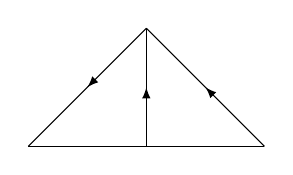
\begin{tikzpicture}[scale=.75]
      \draw (-4,0) -- (-2,0);
      \draw[middlearrow={latex}] (-2,0) -- (-4,2);
      \draw[middlearrow={latex}]  (-4,0) -- (-4,2);

      \draw (-6,0) -- (-4,0);
      \draw[middlearrow={latex}] (-4,2) -- (-6,0);
    \end{tikzpicture}
  \end{center}
  Unattaching if we break this up along the perpindicular and reattach
  preserving the edge identifications we get the space
  \begin{center}
    \begin{tikzpicture}[scale=1.5]
      \draw (0,0) -- (1,0);
      \draw[middlearrow={latex}] (1,0) -- (1,1);
      \draw (1,1) -- (0,1);
      \draw[middlearrow={latex}] (0,1) -- (0,0);
    \end{tikzpicture}
  \end{center}
  From the last image it is clear that the resulting space $X$ is the
  M\"{o}bius band.
\end{solution}

\begin{exercise}{2.1.3}{\parindent}
  Construct a $\Delta$-complex structure on $\R P^n$ as a quotient of a
  $\Delta$-complex structure on $S^n$ having two vectors of length 1
  along each coordinate axis in $\R^{n+1}$.
\end{exercise}
\begin{solution}{\parindent}
  The $\Delta$-complex structure on $S^n$ is given as follows:
  \begin{enumerate}
  \item For each basis vector $e_j$ in $\R^{n+1}$ we create two
    vertices $v_{j,0},v_{j,1}$ corresponding to $\pm e_j$,
    respsectively.
  \item For each $n$-subset of the $\{v_{j,k}\}$ create an $n$-simplex
    and attach it along the set of vertices
    $\{v_{1,k_1},\ldots,v_{n,k_n}\}$. Geometrically, this will add an
    $n$-simplex for each quadrant of $\R^{n+1}$.
  \item At this point we have $2^{n+1}$ $n$-simplices, and the
    resulting space is clearly homeomorphic to $S^{n}$ by just pushing
    out the faces.
  \end{enumerate}
  Now, to get the resulting $\Delta$-complex structure on $\R P^{n}$,
  we identify opposite points, so we set
  \[
  (v_{1,j}, v_{2,j}, \ldots, v_{n,j}) \sim (v_{1,j'}, v_{2,j'},
  \ldots, v_{n,j'})
  \]
  with $j' = j+1 \mod 2$. This space is clearly homeomorphic $\R P^{n}$
  because we have identified opposite points in $S^n$.
\end{solution}

\begin{exercise}{2.1.4}{\parindent}
  Compute the simplicial homology groups of the triangular patachute
  obtained from $\Delta^2$ by identifying its three vertices to a
  single point.
\end{exercise}
\begin{solution}{\parindent}
  After identifying the vertices, we are left with the following
  $\Delta$-complex:
  \begin{center}
    \begin{tikzpicture}
      % node labels
      \node (v) at (-1,-.2) {$v$};
      \node (v) at (1,-.2) {$v$};
      \node (v) at (0,1.92) {$v$};
      % edge labels
      \node (v) at (0,-.2) {$a$};
      \node (v) at (.75,1) {$b$};
      \node (v) at (-.75,1) {$c$};
      % arrows
      \draw[middlearrow={latex}] (-1,0) -- (1,0);
      \draw[middlearrow={latex}] (1,0) -- (0,1.72);
      \draw[middlearrow={latex}] (0,1.72) -- (-1,0);
    \end{tikzpicture}
  \end{center}
  As we can see, there is one 0-simplex, three 1-simplices, and one
  2-simplex. This leads to the chain complex
  \begin{center}
    \begin{tikzcd}
      0 \arrow{r}{} & \Z \arrow{r}{\partial_2} & \Z \oplus \Z \oplus
      \Z \arrow{r}{\partial_1} & \Z \arrow{r}{\partial_0} & 0
    \end{tikzcd}
  \end{center}
  Where the boundary maps are given by
  \begin{align*}
    \partial_0(v) &= 0 \\
    \partial_1(a) = \partial_1(b) = \partial_1(c) &= 0 \\
    \partial_2(X) &= a + b - c
  \end{align*}
  So the homology groups become
  \begin{align*}
    H_0^{\Delta}(X) &= \ker \partial_0/\im \partial_1 = \Z/0  \Z\\
    H_1^{\Delta}(X) &= \ker \partial_1/\im \partial_0 = (\Z \oplus \Z
    \oplus \Z)/\Z = \Z \oplus \Z \\
    H_2^{\Delta}(X) &= \ker \partial_2/\im \partial_1 = 0/0 = 0 \\
    H_n^{\Delta}(X) &= 0, n > 2
  \end{align*}
\end{solution}

\begin{exercise}{2.1.5}{\parindent}
  Compute the simplicial homology groups of the Klein bottle using the
  $\Delta$-complex structure described at the beginning of this
  section.
\end{exercise}
\begin{solution}{\parindent}
  Recall the $\Delta$-complex structure on the Klein bottle, $K$, is
  given by:
  \begin{center}
    \begin{tikzpicture}
      \draw[middlearrow={latex}] (-1,0) -- (1,0);
      \draw[middlearrow={latex}] (1,2) -- (1,0);
      \draw[middlearrow={latex}] (1,2) -- (-1,2);
      \draw[middlearrow={latex}]  (-1,0) -- (-1,2);
      \draw[middlearrow={latex}] (-1,0) -- (1,2);
      % nodes
      \node (v) at (-1,-.2) {$v$};
      \node (v) at (1,-.2) {$v$};
      \node (v) at (1,2.2) {$v$};
      \node (v) at (-1,2.2) {$v$};
      %edges
      \node (a) at (-1.2,1) {$a$};
      \node (b) at (0,2.2) {$b$};
      \node (a) at (1.2,1) {$a$};
      \node (b) at (0,-.2) {$b$};
      \node (c) at (0,1.25) {$c$};
      % faces
      \node (U) at (-.5,1.5) {$U$};
      \node (L) at (.5,.5) {$L$};
    \end{tikzpicture}
  \end{center}
  So from the above it is clear that we have one 0-simplex, three
  1-simplices, and two 2-simplices. So we have the following exact
  sequence:
  \begin{center}
    \begin{tikzcd}
      0 \arrow{r}{} & \Z\oplus\Z \arrow{r}{\partial_2} & \Z \oplus \Z \oplus
      \Z \arrow{r}{\partial_1} & \Z \arrow{r}{\partial_0} & 0
    \end{tikzcd}
  \end{center}
  We then compute the boundary maps:
  \begin{align*}
    \partial_0(v) &= 0 \\
    \partial_1(a) = \partial_1(b) = \partial_1(c) &= 0 \\
    \partial_2(U) &= a + b - c \\
    \partial_2(L) &= a - b + c
  \end{align*}
  Thus, we see that 
  \[
  \im \partial_2 \cong \lbrace a+b-c, a-b+c \rbrace \cong \lbrace 2a,
  a+b-c\rbrace \cong \Z/2\Z \oplus \Z
  \]
  Using this we see that the homology groups are
  \[
  H_n^{\Delta}(X) =
  \begin{cases}
    \Z & n = 0 \\
    \Z/2\Z \oplus \Z & n = 1 \\
    0 & n \geq 2
  \end{cases}
  \]
\end{solution}

\begin{exercise}{2.1.9}{\parindent}
  Compute the homology groups of the $\Delta$-complex $X$ obtained
  from $\Delta^n$ by identifying all faces of the same
  dimension. Thus, $X$ has a single $k$-simplex for each $k \leq n$.
\end{exercise}
\begin{solution}{\parindent}
  We will show that
  \[
  H_n^{\Delta}(X) =
  \begin{cases}
    \Z & n=0, n\text{ odd} \\
    0 & \text{otherwise}
  \end{cases}
  \]
  Indeed, because there is a unique $k$-simplex for each $k \leq n$ we
  have the chain complex
  \begin{center}
    \begin{tikzcd}
      0 \arrow{r}{} & \Z \arrow{r}{\partial_n} & \Z
      \arrow{r}{\partial_{n-1}} & \ldots \arrow{r}{} &\Z
      \arrow{r}{\partial_0} & 0
    \end{tikzcd}
  \end{center}
  So we only need to compute the boundary maps. Let $\sigma_k$ be the
  unique $k$-simplex in $X$ then
  \[
  \partial_k(\sigma_k) = \sum_{i=0}^{n}(-1)^i\sigma_{k-1} =
  \begin{cases}
    \sigma_{k-1} & n \text{ even} \\
    0 & n \text{ odd}
  \end{cases}
  \]
  So that $\ker \partial_k$ is trivial when $k$ is even and is equal
  to all of $\Z$ when $k$ is odd. Likewise, we see that
  $\im \partial_k \cong \Z$ when $k$ is even and $0$ when $k$ is
  odd.Therefore, we can compute the homology groups as
  \[
  H_k^{\Delta}(X) = \ker \partial_k/\im \partial_{k+1} =
  \begin{cases}
    \Z & k = 0 \\
    0 & k \leq n \text{ even} \\
    0 & k < n \text{ odd} \\
    \Z & k = n \text{ odd}
  \end{cases}
  \]
\end{solution}

\begin{exercise}{2.1.11}{\parindent}
  Show that if $A$ is a retract of $X$ then the map $H_n(A) \to
  H_n(X)$ induced by the inclusion $A \subset X$ is injective.
\end{exercise}
\begin{solution}{\parindent}
  Because $A$ is a retract of $X$ we have that there is a map $r: X
  \to X$ such that $r\mid_A = 1_A$. So we have that maps
  \begin{center}
    \begin{tikzcd}
      A \arrow{r}{i} & X \arrow{r}{r} & A
    \end{tikzcd}
  \end{center}
  as well as the induced homomorphisms of the homology groups
  \begin{center}
    \begin{tikzcd}
      H_n(A) \arrow{r}{i_\ast} & H_n(X) \arrow{r}{r_\ast} & H_n(A)
    \end{tikzcd}
  \end{center}
  Then we note that because $(ri)_\ast = r_\ast i_\ast$ that
  $(ri)_\ast = (1_{H_n(A)})_\ast$. The identity function is clearly an
  isomorphism and so $i_\ast$ must be injective.
\end{solution}

\begin{exercise}{2.1.12}{\parindent}
  Show that a homotopy of chain maps is an equivalence relation.
\end{exercise}
\begin{solution}{\parindent}
  We will say that $f \sim g$ if there is a chain homotopy between
  them. We will first show that the relation $\sim$ is
  reflexive. Indeed, let $F$ be the sequence of trivial homomorphisms
  (all 0 maps) then we see that for a map $f: X \to Y$ we have
  \[
  f_{\#} - f_{\#} = \partial 0 + 0\partial = \partial F + F\partial
  \]
  and so $f \sim f$. Next, suppose that $f \sim g$, we need to show
  that $g \sim f$. By assumption we have a chain homotopy $F$ between
  $f$ and $g$ and so $\partial F + F \partial = f_{\#} - g_{\#}$. To
  compute the other direction we multiply this identity by $-1$ yielding
  \[
  g_{\#} - f_{\#} = -\partial F + (-F)\partial = \partial (-F) +
  (-F)\partial
  \]
  and so $-F$ is the desired chain homotopy between $f$ and
  $g$. Finally, wee need to show transitivity. Suppose that $f \sim g$
  and $g \sim h$, so that there are chain homotopies $F_0,F_1$ such
  that $f_{\#} - g_{\#} = \partial F_0 + F_0\partial$ and $g_{\#} -
  h_{\#} = \partial F_1 + F_1\partial$, respectively. Then we can compute
  \begin{align*}
    f_{\#} - h_{\#} & = f_{\#} - g_{\#} +g_{\#} - h_{\#} \\
    &= \partial F_0 + F_0\partial + \partial F_1 + F_1\partial \\
    &= \partial(F_0 + F_1) + F_0\partial + F_1\partial \\
    &= \partial(F_0 + F_1) + (F_0 + F_1)\partial
  \end{align*}
  Where the third equality follows because $\partial$ is a
  homomorphism, and the fourth equality follows from the definition of
  $F_0+F_1$. Thus, $F_0+F_1$ is the desired chain homotopy, verifying
  that $\sim$ is an equivalence relation.
\end{solution}

\begin{exercise}{2.1.15}{\parindent}
  For an exact sequence $A \to B \to C \to D \to E$ show that $C = 0$
  iff the map $A \to B$ is surjective and the map $D \to E$ is
  injective. Hence, for a pair of space $(X,A)$, the inclusion $A
  \into X$ induces isomorphisms on all homology groups iff $H_n(X,A) =
  0$ for all $n$.
\end{exercise}
\begin{solution}{\parindent}
  First we will give each of the maps a name. Suppose that
  \begin{center}
    \begin{tikzcd}
      A \arrow{r}{\alpha_0} & B \arrow{r}{\alpha_1} & C
      \arrow{r}{\alpha_2} & D \arrow{r}{\alpha_3} & E
    \end{tikzcd}
  \end{center}
  is our exact sequence.In the forward direction we suppose that $C =
  0$. Then we decompose the exact sequence above into two short eact
  sequences
  \begin{center}
    \begin{tikzcd}
      A \arrow{r}{\alpha_0} & B \arrow{r}{\alpha_1} & 0 \\
      0 \arrow{r}{\alpha_2} & D \arrow{r}{\alpha_3} & E
    \end{tikzcd}
  \end{center}
  The first says that $\alpha_0$ must be surjective and the latter
  says that $D \to E$ is injective (c.f. page 114) as desired.

  In the reverse direction we suppose that the sequence is exact and
  that $\alpha_0: A \to B$ and $\alpha_3: D \to E$ are surjective and
  injective, respectively. Because $\alpha_3$ is an injective
  homomorphism, it must have trivial kernel. Moreover, because the
  sequence is exact we have that $\ker \alpha_3 = \im \alpha_2 =
  0$. Because the image of $\alpha_2$ is trivial, it must be the
  trivial homomorphism and so $\ker \alpha_2 = C$. Now we note that
  because $\alpha_0$ is surjective and $\im \alpha_0 = \ker \alpha_1 =
  B$. Because $\ker \alpha_1 = B$ we have that $\im \alpha_1 =
  0$. Combining these two facts gives that $C = 0$.

  Thus, for a pair of spaces $(X,A)$ there long exact sequence of
  homology groups
  \begin{center}
    \begin{tikzcd}
      \cdots \arrow{r}{} H_n(A) \arrow{r}{i_\ast} & H_n(X)
      \arrow{r}{j_\ast} & H_n(X,A) \arrow{r}{\partial} & H_{n-1}(A)
      \arrow{r}{i_\ast} & H_{n-1}(X) \arrow{r}{} & \cdots
    \end{tikzcd}
  \end{center}
  Now because the inclusion maps are always injective, if $i_\ast$ is
  an isomorphism i.e. surjective then we apply the above to see that
  $H_n(X,A) = 0$ for all $n$, and conversely. 
\end{solution}

\begin{exercise}{2.1.16}{\parindent}
  \vspace{-20px}
  \begin{enumerate}
  \item Show that $H_0(X,A) = 0$ iff $A$ meets each path-component of
    $X$.
  \item Show that $H_1(X,A) = 0$ iff $H_1(A) \to H_1(X)$ is surjective
    and each path-component of $X$ contains at most one path-component
    of $A$.
  \end{enumerate}
\end{exercise}
\begin{solution}{\parindent}
  \begin{enumerate}
  \item We begin by showing that there is only one homology class in
    $H_0(X)$ for each path-component of $X$. Indeed, suppose that
    $x_0,x_1$ are points in the same path-component of $X$. Then we
    can find a path $\alpha$ whose endpoints are $x_0,x_1$,
    respectively, and so $\alpha$ is a singular 1-simplex such that
    $\partial \alpha = x_1 - x_0$. Hence, $x_0$ and $x_1$ are
    homologous in $H_0(X)$.

    Proceeding with the forward direction of the problem, suppose that
    $H_0(X,A) = 0$. If we look at the long exact sequence of the pair
    we see
    \begin{center}
      \begin{tikzcd}
        \cdots \arrow{r}{} & H_0(A) \arrow{r}{i_\ast} & H_0(X)
        \arrow{r}{j_\ast} & H_0(X,A) \arrow{r}{} & 0
      \end{tikzcd}
    \end{center}
    Our assumption that $H_0(X,A) = 0$ along with exactness of the
    sequence implies that $i_\ast$ is surjective. Thus the inclusion
    $A \to X$ induces an isomorphism on $H_0$ and by the previous
    discussion, $A$ must intersect each path-component of $X$.

    Conversely, suppose that $A$ intersects each path-component of
    $X$. For each path component of $X$ we can find an $x \in X$ that
    is homologous in $H_0(X)$ to an $a \in A$. Thus the induced map
    $i_\ast(a) = [a] = [x]$ where $[x]$ is the homology class of $X$
    in $H_0(X)$. So $i_\ast$ is surjective. Then if we look at
    \begin{center}
      \begin{tikzcd}
        H_0(A) \arrow{r}{i_\ast} & H_0(X) \arrow{r}{j_\ast} &
        H_0(X,A)\arrow{r}{} & 0
      \end{tikzcd}
    \end{center}
    Then exactness of the short exact sequence above (a subsequence of
    the long exact sequence of the pair) combined with the
    surjectivity of $i_\ast$ imply that $\ker j_\ast = H_0(X)$, and
    consequently $\im j_\ast = 0$. Using exactness again on the zero
    map at the end of the sequence gives that 
    \[
    \ker 0 = H_0(X,A) = 0 = \im j_\ast
    \]
    as desired.
  \item We proceed in a similar manner as the previous part. If we
    look at the long exact sequence of the pair we get
    \begin{center}
      \begin{tikzcd}
        \cdots \arrow{r}{} & H_1(A) \arrow{r}{i_\ast} & H_1(X)
        \arrow{r}{j_\ast} & H_1(X,A) \arrow{r}{\partial} & H_0(A)
        \arrow{r}{} & \cdots
      \end{tikzcd}
    \end{center}
    If we assume that $H_1(X,A) = 0$ then we see that $\ker j_\ast =
    H_1(X)$. By exactness this says that $\im i_\ast = H_1(X)$ and so
    $i_\ast$ is injective. Moreover, we still have that
    \begin{center}
      \begin{tikzcd}
        H_1(X,A)=0 \arrow{r}{\partial} & H_0(A) \arrow{r}{i_\ast} &
        H_0(X) \arrow{r}{} & \cdots
      \end{tikzcd}
    \end{center}
    Which says that $i_\ast$ is injective. Applying the claim at the
    beginning of the previous part, this says that distict path
    components of $A$ map into distinct path components in $X$. Thus,
    each path component in $X$ contains at most one path-component
    of $A$.

    In the reverse direction, suppose that $i_\ast: H_1(A) \to H_1(X)$
    is surjective and that each path component of $X$ contains at most
    path-component of $A$. We again consider the segment of the
    sequence
    \begin{center}
      \begin{tikzcd}
        H_1(X,A) \arrow{r}{\partial} & H_0(A) \arrow{r}{i_\ast} &
        H_0(X) \arrow{r}{} & \cdots
      \end{tikzcd}
    \end{center}
    As before, we apply the claim at the beginning of the previous
    part to conclude that $i_\ast$ is injective and so $\ker i_\ast =
    0$. Using exactness of the long exact sequence we see that
    $\im \partial = 0$. We assumed that $i_\ast: H_1(A) \to H_1(X)$
    was surjective and so $\im i_\ast = H_1(X)$ and by exactness we
    see that $\ker j_\ast = H_1(X)$. Because $j_\ast$ is a
    homomorphism we see that $\im j_\ast = 0$. We then compile these
    facts to see that $\im \partial = \ker \partial = 0$ and so
    $H_1(X,A) = 0$.
  \end{enumerate}
\end{solution}

\begin{exercise}{2.1.18}{\parindent}
  Show that for the subspace $\Q \subset \R$ the relative homology
  group $H_1(\R,\Q)$ is free abelian and find a basis.
\end{exercise}
\begin{solution}{\parindent}
  Because $\Q \subset \R$ we can find a long exact sequence in the
  homology groups
  \begin{center}
    \begin{tikzcd}
      \cdots \to H_{n}(\Q) \arrow{r}{i_\ast} & H_{n}(\R)
      \arrow{r}{j_\ast} & H_{n}(\R,\Q) \arrow{r}{\partial} &
      H_{n-1}(\Q) \arrow{r}{i_\ast} & H_{n-1}(\Q) \to \cdots
    \end{tikzcd}
  \end{center}
  Restricting this sequence and terminating with 0 we get a short
  exact sequence
  \begin{center}
    \begin{tikzcd}
      0 \arrow{r}{} & H_{1}(\R,\Q) \arrow{r}{\partial} & H_{0}(\Q)
      \arrow{r}{i_\ast} & H_{0}(\R) \arrow{r}{} & 0
    \end{tikzcd}
  \end{center}
  Now we apply Proposition 2.6 to compute the homology groups
  $H_0(\Q)$ and $H_0(\R)$ by making a generator for each path
  component. Consequently, we have 
  \[
  H_0(\Q) = \bigoplus_{q \in \Q} \Z, H_0(\R) = \Z
  \]
  So the above resolves to the exact sequence
  \begin{center}
    \begin{tikzcd}
      0 \arrow{r}{} & H_{1}(\R,\Q) \arrow{r}{\partial} & \bigoplus_{q
        \in \Q} \Z \arrow{r}{i_\ast} & \Z \arrow{r}{} & 0
    \end{tikzcd}
  \end{center}
  Now we apply exactness of the sequence to conclude that
  $\ker \partial = 0$ and $\partial$ is injective. Thus, $H_1(\R, \Q)$
  is a subgroup of a free group and therefore, free.

  Now we need to compute a basis. The elements of $C_1(\R,\Q)$
  consists of cycles in $\R$ whose boundaries lie in $\Q$. Therefore,
  the boundary map sends them to some interval $[r_1,r_2]$ with $r_2 -
  r_1 \in \Q$ or to some point $p$ (i.e. $r_1 = r_2$). The boundaries
  are such that if we have a map $\sigma \in C_2(\R,\Q)$ then its
  boundary is some cycle $\varphi = \partial_2\sigma$. So if $\varphi
  \neq 0$ then we must have that $\partial \sigma: \partial\Delta^2
  \to \R$ maps to an an interval $[r_1,r_2]$ such that $r_2-r_1 \in
  \Q$ or it maps to a point that is not in $\Q$.

  By the above discussion we see that $\im \partial_2$ differs from
  $\ker \partial_1$ only on maps $\varphi: \Delta^1 \to \R$ that map
  to a point. Thus, we see that
  \[
  H_1(\R,\Q) = \lbrace \varphi:\Delta^1 \to \R \mid \im \varphi \in
  \Q\rbrace \cong \Q
  \]
  Where the last identification just identifies a $q \in \Q$ with the
  singular simplex $\varphi$ that maps onto $\Q$. Thus, any basis for
  $\Q$ as an additive group will be a basis for $H_1(\R,\Q)$ for
  example, the elements $1,1/2,1/3,\ldots$.
\end{solution}

\begin{exercise}{2.1.22}{\parindent}
  Prove by induction on dimension the following facts about the
  homology of a finite dimensional CW complex X, using the observation
  that $X^n/X^{n-1}$ is a wedge sum of $n$ spheres:
  \begin{enumerate}
  \item If $X$ has dimension $n$ then $H_i(X) = 0$ for $i > n$ and
    $H_n(X)$ is free.
  \item $H_n(X)$ is free with basis in bijective correspondence with
    the $n$-cells if there are no cells of dimension $n-1$ or $n+1$.
  \item If $X$ has $k$ $n$-cells, then $H_n(X)$ is generated by at most
    $k$ elements.
  \end{enumerate}
\end{exercise}
\begin{solution}{\parindent}
  \begin{enumerate}
  \item Following the hint, we proceed by induction. For the case
    $n=0$ note that if there are $k$ 0-cells in $X$ then $H_0(X) =
    \bigoplus_{i=1}^k \Z$, the free abelian group of rank $k$. Also,
    we see that $H_k(X) = 0$ for $k > 0$ because $C_k(X) = 0$ for $k >
    0$.

    For the inductive step suppose that any $(n-1)$-dimensional
    CW-complex $A$ satisfies the proposition, so $H_k(A) = 0$ for $k >
    n-1$ and $H_{n-1}(A)$ is free. For the first part of the claim we
    observe that there are no $k$-cells for $k > n$ and so $C_k(X) =
    0$ for $k > n$ and as a result $H_k(X) = 0$. For the second part
    of the claim we look at the pair $(X,A)$ for an
    $(n-1)$-dimensional subcomplex $A$. There is a long exact sequence
    of the pair
    \begin{center}
      \begin{tikzcd}
        \cdots \to H_{n+1}(A) \arrow{r}{i_\ast} & H_{n+1}(X)
        \arrow{r}{j_\ast} & H_{n+1}(X,A) \arrow{r}{\partial} &
        H_{n}(A) \arrow{r}{i_\ast} & H_{n}(X) \to \cdots
      \end{tikzcd}
    \end{center}
    Then we note that the space $X/A$ is a wedge of $n$-spheres and
    therefore has a $\Delta$-complex structure on it and is a good
    pair. Thus, we can apply Proposition 2.22 to get that $H_n(X,A)
    \cong H_n(X/A)$. This fact along with the inductive hypothesis
    yields the exact sequence
    \begin{center}
      \begin{tikzcd}
        0 \arrow{r}{} & H_{n+1}(X/A) \arrow{r}{} & 0 \arrow{r}{i_\ast}
        & H_{n}(X) \arrow{r}{j_\ast} & H_n(X/A) \arrow{r}{\partial} &
        F
      \end{tikzcd}
    \end{center}
    Where $F$ is a free group. Now we use exactness, noting that $\im
    i_\ast = \ker j_\ast = 0$. So we can use the first isomorphism
    theorem to see that
    \[
    \im j_\ast \cong H_n(X)/\ker j_\ast = H_n(X)
    \]
    Now we use exactness again to conclude that $\im j_\ast \cong
    \ker \partial$ and so $H_n(X) \cong \ker \partial$. However, we
    note that because $\ker \partial$ is the kernel of a homomorphism
    it must be isomorphic to a subgroup of $F$, a free group. Because
    subgroups of free groups of free (Theorem 1A.4) we see that
    $H_n(X)$ must be free as claimed. This completes the induction.
  \item Suppose that there are no cells in $X$ of dimension $(n-1)$ or
    $(n+1)$. Moreover, suppose $X$ has exactly $k$ $n$-cells so that
    the chain complex
    \begin{center}
      \begin{tikzcd}
        \cdots \arrow{r}{} & C_{n+1}(X) \arrow{r}{\partial_{n+1}} &
        C_{n}(X) \arrow{r}{\partial_{n}} & C_{n}(X)
        \arrow{r}{\partial_{n}} & \cdots
      \end{tikzcd}
    \end{center}
    resolves to
    \begin{center}
      \begin{tikzcd}
        \cdots \arrow{r}{} & 0 \arrow{r}{\partial_{n+1}} &
        \bigoplus_{i=0}^k \Z \arrow{r}{\partial_{n}} & 0
        \arrow{r}{\partial_{n}} & \cdots
      \end{tikzcd}
    \end{center}
    because there are no generators for $C_{n+1}$ and $C_{n-1}$ but
    $k$ generators for $C_n$. Then we see that $\im \partial_{n+1} =
    0$ and $\ker \partial_n = \bigoplus_k \Z$. So $H_n(X) =
    \bigoplus_k \Z$ is free with $k$ basis elements and so they can be
    put in bijective correspondence with the $k$ $n$-cells that make
    up the $n$-skeleton of $X$.
  \item Again we will proceed by induction. For the base case $n=0$
    suppose that $X$ has $k$ 0-cells. Then we see that $H_0(X) \cong
    \bigoplus_k\Z$ because there are $k$ components. For the inductive
    step suppose that $H_i(X)$ is generated by at most $k$ elements if
    there are $k$ $i$-cells in $X$. By the discussion in the first
    part of this problem we have a long exact sequence
    \begin{center}
      \begin{tikzcd}
        \cdots \to H_{n}(X^{n-1}) \arrow{r}{i_\ast} & H_{n}(X^n)
        \arrow{r}{j_\ast} & H_{n}(X^n/X^{n-1}) \arrow{r}{\partial} &
        H_{n-1}(A) \arrow{r}{i_\ast} & \cdots
      \end{tikzcd}
    \end{center}
    where $X^n$ is the $n$-skeleton of $X$. Applying the first part of
    this exercise and the inductive hypothesis, we get an exact
    sequence
    \begin{center}
      \begin{tikzcd}
        \cdots \to 0 \arrow{r}{i_\ast} & H_{n}(X^n) \arrow{r}{j_\ast}
        & \bigoplus_k \Z\arrow{r}{} & \cdots
      \end{tikzcd}
    \end{center}
    We know that $\im i_\ast = 0$ and so $H_n \cong \ker j_\ast$. Then
    notice that $\ker j_\ast$ is a subgroup of a free group with $k$
    generators. Thus, it is free with at most $k$ generators. Because
    $X$ is $n$-dimensional we see that $H_n(X) \cong H_n(X^n) \cong
    \bigoplus_\ell \Z$ where $\ell \leq k$ as desired.
\end{enumerate}
\end{solution}

\begin{exercise}{2.1.26}{\parindent}
  Show that $H_1(X,A)$ is not isomorphic to $\tilde{H}_1(X/A)$ if $X =
  [0,1]$ and $A$ is the sequence $1,1/2,1/3,\ldots$ together with its
  limit 0.
\end{exercise}
\begin{solution}{\parindent}
  First we will show that the relative homology group $H_1(X,A)$ is
  countable. Indeed, consider the long exact sequence of homology
  groups given by the inclusion:
  \begin{center}
    \begin{tikzcd}
      \cdots \to H_{n}(A) \arrow{r}{i_\ast} & H_{n}(X)
      \arrow{r}{j_\ast} & H_{n}(X,A) \arrow{r}{\partial} &
      H_{n-1}(A) \arrow{r}{i_\ast} & H_{n-1}(X) \to \cdots
    \end{tikzcd}
  \end{center}
  Restricting this sequence to a short exact sequence terminating in
  zeros we get a short exact sequence like
  \begin{center}
    \begin{tikzcd}
      0 \arrow{r}{} & H_{1}(X,A) \arrow{r}{\partial} & H_0(A)
      \arrow{r}{i_\ast} & H_0(X) \arrow{r}{} & 0
    \end{tikzcd}
  \end{center}
  We then apply Proposition 2.6 to see that $H_0(A) = \bigoplus_{n\in
    \N} \Z$ and $H_0(X) = \Z$. Consequently, the above becomes the
  sequence
  \begin{center}
    \begin{tikzcd}
      0 \arrow{r}{} & H_{1}(X,A) \arrow{r}{\partial} & \bigoplus_{n\in
        \N} \Z \arrow{r}{i_\ast} & \Z \arrow{r}{} & 0
    \end{tikzcd}
  \end{center}
  Then exactness implies that $\partial$ is injective and so 
  \[
  H_1(X,A) \leq \bigoplus_{n \in \N} \Z
  \]
  In particular, this implies that $H_1(X,A)$ is countable.

  Now we will compute the reduced homology group
  $\tilde{H}_1(X/A)$. We see that the space $X/A$ is the familiar
  Hawaiian earring. Following the notation in Example 1.25 we let
  $C_n$ be the circle of radius $1/n$ and center $(0,1/n)$. Each of
  the retractions $r_n: X/A \to C_n$ induces a homomorphism on the
  homology $(r_n)_\ast: \tilde{H}_1(X/A) \to \tilde{H}_1(C_n)$. Now
  recall that the circle $C_n$ only has one path-component and
  therefore $\tilde{H}_1(C_n) \cong \Z$. Now we will see that this
  homomorphism is surjective. If we consider a singular 1-simplex
  $\sigma: \Delta^1 \to X/A$, then it is non-zero because $\sigma(0)
  \neq \sigma(1)$ ($\sigma(0) = 1/n, \sigma(1) = 1/(n+1)$, so it must
  be mapped to a generator of $\tilde{H}_1(C_n)$.

  Now consider the product of each of the $(r_n)_\ast$ which is given
  by $\rho: \tilde{H}_1(X/A) \to \prod_{n=1}^\infty \Z$. This is a
  direct product and not a direct sum because every loop in $X/A$
  corresponds to a distinct sequence of integers. This map must be
  surjective because because there is a singular $1$-simplex
  $\sigma_k: \Delta^1 \to C_n$ any given number of times. So 
  \[
  \prod_{i=1}^\infty \Z \leq \tilde{H}_1(X/A)
  \]
  Because $\prod_{i=1}^\infty \Z$ is uncountable, we see that
  $\tilde{H}_1(X/A)$ is uncountable. Thus, we see that $H_1(X,A)
  \not\cong \tilde{H}_1(X/A)$.
\end{solution}

\begin{exercise}{2.1.29}{\parindent}
  Show that $S^1 \times S^1$ and $S^1 \vee S^1\vee S^2$ have
  isomorphic homology groups in all dimensions, but their universal
  covering spaces do not.
\end{exercise}
\begin{solution}{\parindent}
  We know that the homology groups of $S^1 \times S^1$ are
  \[
  H_n(S^1 \times S^1) =
  \begin{cases}
    \Z \oplus \Z & n = 1 \\
    \Z & n = 0,2 \\
    0 & n \geq 3
  \end{cases}
  \]
  Now, we apply Corollary 2.25 to see that the inclusions $S_1 \to
  (S^1\vee S^1\vee S^2)$ induce an isomorphism
  \[
  \varphi: H_n(S^1) \oplus H_n(S^1) \oplus H_n(S^2) \lra H_n(S^1\vee
  S^1\vee S^2)
  \]
  Then we use the fact that
  \[
  H_k(S^n) =
  \begin{cases}
    \Z \oplus \Z & n=k=0 \\
    \Z & k = 0 \\
    0 & 0 < k < n \\
    \Z & k = n
  \end{cases}
  \]
  So that
  \[
  H_k(S^1\vee S^1\vee S^2) =
  \begin{cases}
    \Z \oplus \Z & k = 0\\
    \Z & k = 1 \\
    0 & k \geq 2
  \end{cases}
  \]
  Now we compute the homology of the universal covering spaces. We
  know that the universal cover of $S^1 \times S^1$ is $\R \times
  \R$. And in particular we see that $H_2(\R \times \R) = 0$ because
  $\R$ is contractible. Suppose that $p:\tilde{X} \to S^1\vee S^1\vee
  S^2$ is the universal cover and consider the inclusion $i: S^2 \to
  \tilde{X}$. The inclusion must factor through the universal
  cover. Then the induced map $i_\ast: H_2(S^2) \to H_2(S^1\vee
  S^1\vee S^2)$ is injective and factors through a map in the homology
  group of the universal cover leading to the diagram
  \begin{center}
    \begin{tikzcd}
      & H_2(\tilde{X}) \arrow{d} \\
      H_2(S^2) \cong \Z \arrow{r}{i_\ast} \arrow{ru} & H_2(S^1\vee
      S^1\vee S^2)
    \end{tikzcd}
  \end{center}
  Therefore $H_2(\tilde{X})$ is non-zero and we are done.
\end{solution}

\begin{exercise}{2.1.30}{\parindent}
  In each of the following commutative diagrams assume that all maps
  but one are isomorphisms. Show that the remaining map must be an
  isomorphism as well.
  \begin{center}
    \begin{tikzcd}
      A \arrow{r} \arrow{dr} & B \\
      & C \arrow{u}
    \end{tikzcd}
    \begin{tikzcd}
      A \arrow{r} \arrow{d} & B \arrow{d} \\
      C \arrow{r} & D
    \end{tikzcd}
    \begin{tikzcd}
      A \arrow{d} \arrow{r} & B \\
      C \arrow{r} & D \arrow{u}
    \end{tikzcd}
  \end{center}
\end{exercise}
\begin{solution}{\parindent}
  For the first diagram, we give the functions names to make this more
  clear. We have
  \begin{center}
    \begin{tikzcd}
      A \arrow{r}{f} \arrow{dr}{g} & B \\
      & C \arrow{u}{h}
    \end{tikzcd}
  \end{center}
  Commutativity implies that $f = hg$. There are three cases
  \begin{enumerate}
  \item If $h,g$ are isomorphisms, then the commutativity of the
    diagram forces $f$ to be an isomorphism because the composition of
    isomorphisms is an isomorphism.
  \item If $f,h$ are isomorphisms then we apply $h^{-1}$ to both sides
    to get the equality $g = h^{-1}f$. Thus, $g$ is a composition of
    isomorphisms and therefore and isomorphisms.
  \item In the final case we have that $f,g$ are isomorphisms. Then we
    precompose both sides with $g^{-1}$ yielding $h = fg^{-1}$ and so
    $h$ is an isomorphism.
  \end{enumerate}

  For the second diagram we have
  \begin{center}
    \begin{tikzcd}
      A \arrow{r}{f} \arrow{d}{g} & B \arrow{d}{g'} \\
      C \arrow{r}{f'} & D
    \end{tikzcd}
  \end{center}
  Commutativity gives the equation $g'f = f'g$. Much in the same
  manner as the last problem we will compose with the correct inverse
  in order to obtain the excluded map as a composition of three
  isomorphisms, and thus, it must be an insomorphism as well.
  \begin{enumerate}
  \item If we are looking for $f$, we note that $f = (g')^{-1}f'g$.
  \item For $g$ we see that $g = (f')^{-1}g'f$.
  \item Likewise for $f'$ we see that $f' = g'fg^{-1}$.
  \item Finally for $g'$ we see that $g' = f'gf^{-1}$.
  \end{enumerate}
  For the last diagram, we do exactly the same thing. We start with
  \begin{center}
    \begin{tikzcd}
      A \arrow{d}{g} \arrow{r}{f} & B \\
      C \arrow{r}{f'} & D \arrow{u}{g'}
    \end{tikzcd}
  \end{center}
  Yielding the equation $(g')^{-1}f = f'g$. So we have
  \begin{enumerate}
  \item If we are looking for $f$, we note that $f = g'f'g$.
  \item For $g$ we see that $g = (f')^{-1}(g')^{-1}f$.
  \item Likewise for $f'$ we see that $f' = (g')^{-1}fg^{-1}$.
  \item Finally for $g'$ we see that $(g')^{-1} = f'gf^{-1}$. So $g' =
    fg^{-1}(f')^{-1}$.
  \end{enumerate}
\end{solution}

\begin{exercise}{2.1.31}{\parindent}
  using the notation of the five-lemma, give an example where the maps
  $\alpha, \beta, \delta, \epsilon$ are zero but $\gamma$ is
  non-zero. This can be done with short exact sequences in which all
  the groups are either $\Z$ or 0.
\end{exercise}
\begin{solution}{\parindent}
  Following the hint, we will find a commutative diagram as in the
  Five-Lemma using only $\Z$ and 0 as the groups. Indeed, consider the
  diagram:
  \begin{center}
    \begin{tikzcd}
      \Z \arrow{r}{0} \arrow{d}{0} & 0 \arrow{r}{i} \arrow{d}{0} & \Z
      \arrow{r}{\approx} \arrow{d}{\approx}& \Z \arrow{r}{0}
      \arrow{d}{0}&
      0 \arrow{d}{0} \\
      0 \arrow{r}{i} & \Z \arrow{r}{\approx} & \Z \arrow{r}{0} & 0
      \arrow{r}{0} & 0
    \end{tikzcd}
  \end{center}
  where $\approx$ signifies an isomorphism. Each of the rows is easily
  checked to be exact and moreover, the diagram commutes. Thus, this
  is an example of such a diagram.
\end{solution}
\end{document}